\documentclass{beamer}
\usetheme[progressbar=frametitle]{metropolis}
\usepackage[utf8]{inputenc}

\usepackage{booktabs}
\usepackage[scale=2]{ccicons}
\usepackage[export]{adjustbox}
\usepackage{pgfplots}
\usepackage{fancyhdr}
\usepackage{amsmath,amssymb,wrapfig,amsfonts,amsbsy,amssymb,amstext,mathrsfs,latexsym,amsthm,mathtools}
\usepgfplotslibrary{dateplot}
\usepackage[backend=bibtex,style=authoryear,natbib=true]{biblatex}
\usepackage{xspace}
\newcommand{\themename}{\textbf{\textsc{metropolis}}\xspace}
\DeclareUnicodeCharacter{211D}{$\mathbb{R}$}

\addbibresource{biblio.bib}

\title{Capstone Presentation}
\subtitle{The Duality Principle for Unitary Systems}
\author{Naman Vishal Kedia}
\date{April 2023}

\begin{document}

\maketitle

\begin{frame}{Table of contents}
  \setbeamertemplate{section in toc}[sections numbered]
  \tableofcontents%[hideallsubsections]
\end{frame}

% \section[A Motivating Example]{A Motivating Example}

% \begin{frame}[fragile]{Music Recognition}

%     
\includegraphics[height=1cm]{shazamlogo.png}
%     
\includegraphics[height = 1cm]{soundhound2.png}

%   Music Recognition programs such as Shazam and Soundhound store music in the form of digital fingerprints and use a matching algorithm in order to match this digital fingerprint against a database of songs for which the fingerprints have already been created.

%   In order to understand the process of digital fingerprinting, we must look at the Fourier Transform and specifically the Gabor Transform, also known as the Short Term Fourier Transform.
% \end{frame}

\section{Motivation}

\begin{frame}{Literature Review Summary}

\textbf{\cite{dai1998wandering}} - Introduce wandering vectors, use von-Neumann algebras to study wavelet systems.

\textbf{\cite{HL2000}} - Dilation view of frames, prove main result of this capstone using von-Neumann algebras

\textbf{\cite{ron1995frames}} - Introduce duality principle for Gabor frames.

\textbf{\cite{fan2016dual}} \& \textbf{\cite{Fan2016}} - Introduce dual Gramian analysis and duality principle for Hilbert spaces and for frames.
    
\end{frame}


\begin{frame}{Project Overview}

\begin{enumerate}
    \item While performing a literature review, I recognised the need for an \textbf{accessible introduction} to the duality principle and frames beyond what is provided in the aforementioned literature and in books such as \textbf{\cite{christensen2008frames}}. Therefore this project aimed to provide such an introduction without requiring extensive background knowledge. 
    \item The project also aimed to provide approaches to proving a result relating to \textbf{unitary systems} which have a \textbf{wandering vector} using the \textbf{duality principle}. The result, proved in \textbf{\cite{HL2000}}, is given in the following slide.
\end{enumerate}
\end{frame}

\begin{frame}{Main Result}
    \textbf{Let $\pi$ be a projective unitary representation of a group $G$ on $H$, with a wandering vector. Then $\eta\in H$ generates a
\begin{itemize}
    \item[(i)] frame if and only if it generates a Riesz basis.
    \item[(ii)] tight frame if and only if it generates an orthonormal basis.
\end{itemize}}  
\end{frame}

\section{Frames \& the Duality Principle}

\begin{frame}{Orthonormal Basis}
Let $V$ be a vector space equipped with a complex inner product, and $(v_i)_{i = 1}^n \subset V$ be an orthonormal basis for the space. Then for all $x \in V$ the following properties hold true:
    \begin{equation} \label{ortho_prop}
    \langle v_i, v_j \rangle = 
        \begin{dcases*}
        $1,$ & \mbox{if } $i = j$, \\
        $0,$ & \mbox{if } $i \neq j$,
        \end{dcases*}
\end{equation}

\begin{equation} \label{perf_rep_orth}
    x = \sum_{i = 1}^n\langle x, v_i \rangle v_i,
\end{equation}

\begin{equation} \label{parseval_eq}
    \|x\|^2 = \sum_{i = 1}^n |\langle x, v_i \rangle|^2.
\end{equation}
\end{frame}

\begin{frame}{Analysis and Synthesis Operators}
    Let $V$ be a vector space and $X \subset V$ be a system (collection of vectors). Let $W$ be the vector space consisting of sequences of length $\#X$.
    
    The \textbf{analysis operator}, $T^*: V \to W$, is defined with respect to $X$ by 
\begin{equation} \label{analysis}
    T_X^*v = \left(\langle v, x \rangle \right)_{x \in X}, \qquad \forall v \in V,
\end{equation}
and the \textbf{synthesis operator}, $T: W \to V$ is defined with respect to $X$ by
\begin{equation} \label{synthesis}
T_X\left(\alpha(x)\right)_{x \in X} = \sum_{x \in X} \alpha(x) x, \qquad \forall \left(\alpha(x)\right)_{x \in X} \in W.
\end{equation}
\end{frame}

\begin{frame}{Adjoint Systems}
    The \textbf{adjoint system} for a system $X$, given by $X^*$, is the system for which the analysis operator for $X$ is the synthesis operator for the $X^*$ which can be restated as $T_{X^*} = T^*_X$.

    This definition remains consistent with our understanding of the \textbf{adjoint operator} and we see that for all $v \in V$ and for all $ w \in W$, the analysis and synthesis operators of a system are adjoint operators of each other, 
    $$\langle T_Xw, v \rangle_V = \langle w, T_X^*v \rangle_W.$$
\end{frame}

\begin{frame}{Gramians and dual Gramians}
    A matrix representation of the synthesis operator for a system is called a \textbf{pre-Gramian} denoted by $\mathcal{J}_X$. Matrix representations of the operators $T_X^*T_X$ and $T_XT_X^*$ are called \textbf{Gramians} and \textbf{dual Gramians} and are given by $\mathcal{J}^*_X\mathcal{J}_X$ and $\mathcal{J}_X\mathcal{J}^*_X$ respectively.

    We should also note that a matrix representation of the synthesis operator of a system is given with the columns of the matrix being the vectors of the system. These matrix representations are with respect to a choice of orthonormal basis used to represent them.
\end{frame}

\begin{frame}{Frames \& Riesz Sequences}
    Let $V$ be a vector space and $X \subset V$ be a system. $X$ is a \textbf{frame} if there exist $A, B > 0$, such that for all $v \in V$,
\begin{equation} \label{frameBounds}
    A \| v \|^2 \leq \| T_X^*v \|^2 \leq B\|v\|^2
\end{equation}
where $T_X^*$ is the analysis operator of the system and if $A = B = 1$, then it is known as a \textbf{1-tight frame}.

$X$ is a \textbf{Riesz sequence}, if there exists $C, D > 0$, such that for all $\alpha \in W$,
\begin{equation} \label{RieszBounds}
    C \| \alpha \|^2 \leq \| T_X\alpha \|^2 \leq D\|\alpha\|^2
\end{equation}
where $T_X$ is the synthesis operator of the system. If $C = D = 1$, then it an \textbf{orthonormal Riesz sequence} and if $X$ spans the space then it is a \textbf{Riesz basis}.
\end{frame}

\begin{frame}{Hilbert Spaces}
    \textbf{Hilbert spaces} are complete normed vector spaces with the norm arising from an inner product. They include all finite-dimensional vector spaces as well as some infinite-dimensional vector spaces.
    
    We consider \textbf{separable} Hilbert spaces, which are Hilbert spaces with a countable dense subset in order to find matrix representations for operators in the space. We consider \textbf{Schauder bases} which allow us to consider series instead of finite sums in infinite dimensions. We also extend our definition of analysis and synthesis operators in infinite dimensions to consider systems where $V = H$ and $W = \ell_2(X)$ for Hilbert space $H$ and system $X$. 
\end{frame}

\begin{frame}{Bi-Infinite Matrices}
    Finally, we consider infinte-dimensional matrix representations of synthesis operators in a Hilbert space. Let $K, K'$ be countable index sets,  $(o_{k'})_{k' \in K'}$ be an orthonormal basis for $H$ and $(e_k)_{k \in K}$ be the standard basis for $\ell_2(X)$, then pre-Gramian
    \begin{equation} \label{inf_pre_gram}
    \mathcal{J}_X = \left(\langle Te_k, o_{k'} \rangle \right)_{k' \in K', k \in K} = \left(\langle x_k, o_{k'} \rangle \right)_{k' \in K', k \in K}.
\end{equation}
We require that the rows and columns be square summable in order to ensure convergence of series which form entries of Gramians and dual Gramians.
\end{frame}

\begin{frame}{Matrix Example 1}
The columns of the matrix are an example of a 1-tight frame, 
$$\sqrt{\frac{2}{3}}\left[ \begin{array}{ccc}
       0  & -\frac{\sqrt{3}}{2}  & \frac{\sqrt{3}}{2} \\
       1  & -\frac{1}{2} & -\frac{1}{2}
    \end{array}\right].$$
    
We note that although the rows are orthonormal, they do not span the space $\mathbb{C}^3$. They form an orthonormal Riesz sequence, but not an orthonormal basis.

Note the relationship seen above where the columns of the matrix form a tight frame and the rows form an orthonormal Riesz sequence which provides us with some indication that there might be some relationship between the system of rows and columns of a matrix.
\end{frame}

\begin{frame}{Matrix Example 2}
    Consider the following matrix
    $$\left[ \begin{array}{ccc}
       1  & 2  & 1 \\
       2  & 2 & 3 \\
       1 & 3 & 3
    \end{array}\right]$$
We note that it is a symmetric matrix and this provides us with some indication that there is a relationship between the system of rows of the matrix and the system of columns of the matrix, i.e. they are the same.
\end{frame}

\begin{frame}{The Duality Principle}
     Let $V$ be a Hilbert space with system $X$, then the \textbf{duality principle} states that
    \begin{enumerate}[(i)]
        \item $X$ is a frame if and only if $X^*$ is a Riesz sequence,
        \item $X$ is a 1-tight frame if and only if $X^*$ is an orthonormal Riesz sequence,
    \end{enumerate}
    The duality principle follows directly from the definition of adjoint systems.
    
    The previous examples illustrate specific instances of the duality principle where the columns are formed $X$ and rows formed $X^*$.
\end{frame}

\section{Unitary Systems}

\begin{frame}{Unitary Equivalence and Projective Unitary Representations}
    A \textbf{unitary operator} $U$ is one for which $U^* = U^{-1}$. Two matrices $\mathcal{A}, \mathcal{B}$ are \textbf{unitarily equivalent} if there exists unitary matrix $U$ such that $\mathcal{A} = U\mathcal{B}U^*$. Unitary equivalence is important since it corresponds to a change in orthonormal basis and allows us to consider matrix representations of operators independent to the choice of orthonormal basis.
    
    Let $G$ be a countable group and $H$ be a separable Hilbert space, then we consider the group of consisting of all the unitary operators on this space given by $\mathcal{U}(H)$ and define a \textbf{projective unitary representation} to be a group homomorphism from $\pi: G \to \mathcal{U}(H)$ upto a unimodular multiplier, i.e. for all $g, h \in G$,
    $$\pi(g)\pi(h) = \mu(g,h)\pi(gh), \quad \| \mu(g,h) \| = 1.$$

    
\end{frame}

% \begin{frame}{Some Important Results}
%     Some important results proved in textbooks such as \cite{christensen2008frames} and \cite{ovchinnikov2018functional} that will be referenced are that
%     \begin{itemize}
%         \item Every Riesz basis is a frame.
%         \item 
%     \end{itemize}
% \end{frame}

\begin{frame}{An Original Result}
A vector $\eta\in H$ is called the \textbf{generator} of system $\pi(G)\eta:=(\pi(g)\eta)_{g\in G}$. The generator is called a \textbf{wandering vector}, or complete wandering vector if $\pi(G)\eta$ is an orthonormal basis for $H$ and a \textbf{Riesz vector} if $\pi(G)\eta$ is a Riesz basis.

    Let $\psi$ be a wandering vector for $H$ and $\eta\in H$.
Then for all  $h\in G$, $(\psi_{g,h})_{g\in G}
:=(\overline{\mu(g,g^{-1})}\mu(g^{-1},h)\pi(g^{-1}h)\psi)_{g\in G}$ is shown to be an orthonormal basis for the space. 

This is important since the pre-Gramian with respect to this orthonormal basis is $\mathcal{J}_{\eta}:=(\langle\pi(g)\eta,\pi(h)\psi\rangle)_{h,g\in G}=
(\langle\eta,\psi_{g,h}\rangle)_{h,g\in G},$ which is a simpler formulation of the pre-Gramian and might aid in proving the main result.
\end{frame}

\begin{frame}{Main Result Restated}
    \textbf{Let $\pi$ be a projective unitary representation of a group $G$ on $H$, with a wandering vector. Then $\eta\in H$ generates a
\begin{itemize}
    \item[(i)] frame if and only if it generates a Riesz basis.
    \item[(ii)] tight frame if and only if it generates an orthonormal basis.
\end{itemize}}  
\end{frame}

\section{Approaches}

\begin{frame}{Approach 1: Diagonal Argument}
To understand this argument we first must refer to a result from \textbf{\cite{christensen2008frames}}, which states that every Riesz basis is also a frame.

This argument also relies on $\mathcal{J}_\eta$ being injective which implies that $\mathcal{J}^*_\eta$ is surjective and that the adjoint system is in fact a basis, however, I have not been able to show this yet.

Keeping these results in mind we refer to the argument stated in the following slide, bearing in mind that an analogous idea can be used for the case of frames and Riesz bases.
\end{frame}

\begin{frame}{Approach 1: Diagonal Argument}
    \begin{figure}[H]
\centering
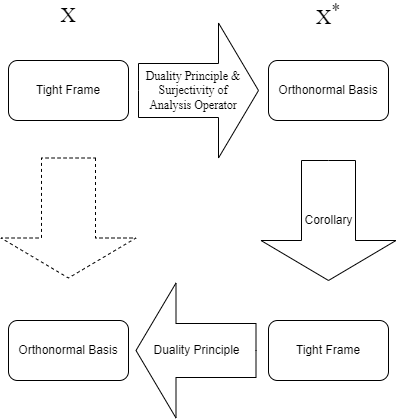
\includegraphics[width=14pc,height=14pc,keepaspectratio]{diagram}
\decoRule
\caption{Diagonal Argument}
\label{fig:diagram}
\end{figure}
\end{frame}

\begin{frame}{Approach 2: Matrix Analysis}
    We note that the inner products in every row and every column of $\mathcal{J}_{\eta}$ contain (up to a unimodular factor) every element of the basis
 $(\psi_{g,h})_{g\in G}$ exactly once. Therefore, by rearranging inner products in a matrix representation if we can show that the system is its own adjoint system up to unitary equivalence, then the result follows from the duality principle.

If we use the extra assumption that $G$ is abelian, and are able to show that up to unitary equivalence,
\[
\left(\langle\eta,\pi(g)\pi(h)\psi\rangle\right)_{h,g} = 
\left(\langle\eta,\mu(g,h)\overline{\mu}(h,g)\pi(h)\pi(g)\psi\rangle\right)_{h, g}.
\]

\end{frame}

\begin{frame}{Approach 2: Matrix Analysis}
    In general, $\mu(g,h)\overline{\mu}(h,g) \neq 1$ however we see in Chapter 4 of \textbf{\cite{HL2000}}, having a wandering vector provides additional structure to the system which may result in $\mu(g,h)\overline{\mu}(h,g) = 1$. Further analysis is required into understanding whether this is true in the given case or not. If it is true, then we see that 
    \[ \mathcal{J}_{\eta} = (\mathcal{J}_{\eta})^\top U.\]

    This can be equivalently done by considering the Gramian and showing that it is the same as the dual Gramian upto unitary equivalence as well.
\end{frame}

\begin{frame}{Approach 3: Co-Isometries}
    The following result is from \textbf{\cite{HL2000}}. Let $C_{\psi}(\mathcal{U}(H))$ refer to the local commutant of the unitary system. Suppose that $\psi$ is a wandering vector for a unitary system $\mathcal{U}(H)$, then \textbf{a vector $\eta$ is a normalized tight frame vector if and only if there exists a unique co-isometry $A \in C_{\psi}(\mathcal{U}(H))$ such that $A\psi = \eta$}. 

    Furthermore another result from \textbf{\cite{dai1998wandering}} states that \textbf{all wandering vectors of a unitary system are unitarily equivalent to one another and these unitary operators are in the local commutant of the system}, and the number of unitary operators in the local commutant is equal to the number of wandering vectors.
\end{frame}

\begin{frame}{Approach 3: Co-Isometries}
 Thus, if we can show that the unique co-isometry $A$ is in fact unitary, we will have shown that $\eta$ is unitarily equivalent to $\psi$ and thus is a wandering vector. 
 
    Proposition 3.5, Corollary 3.6, and the comment following Corollary 3.6 from \textbf{\cite{HL2000}} may be used in order to similarly prove results for (i) of the Main Result. 

This would show that the system generated by $\eta$ would be its own adjoint system and up to unitary equivalence and thus the result would follow due to the duality principle.
\end{frame}

\section[Thank You]{End}

\begin{frame}[allowframebreaks]
        \printbibliography
\end{frame}

\end{document}

% \section{Important Points to Note}
% \begin{frame}{A Symmetric Matrix}
% Consider the following matrix
%     $$\left[ \begin{array}{ccc}
%        1  & 2  & 1 \\
%        2  & 2 & 3 \\
%        1 & 3 & 3
%     \end{array}\right]$$
% We note that it is a symmetric matrix and this provides us with some indication that there is a relationship between the set of rows of a matrix and the set of columns of the matrix, i.e. they are the same.
% \end{frame}



% \section[Short Term Fourier Transform]{Gabor Transform}

% \begin{frame}[fragile]{Fourier Transform}
% The Fourier Transform is an operator which converts signals from the time domain to the frequency domain. Assuming we call this invertible operator $\mathscr{F}$, it is defined for a function $f(x)$ as below:
% $$\mathscr{F}f = \hat{f}(\omega) = \int_{-\infty}^{\infty}{e^{-i\omega x}f(x) \,dx} $$

% This means that the output function, takes in frequency inputs and tells you the intensity of the signal at that frequency. However, a limitation of this is that it is the frequencies are not localized, i.e. it considers the intensity of signals over the entire sound rather than at short time intervals, which is what the Gabor Transform addresses.
% \end{frame}

% \begin{frame}[fragile]{Short Term Fourier Transform}
% The Gabor Transform introduces the idea of a "sliding window", by taking a function $g$ which is square-integrable. Then the Gabor Transform $\mathscr{G}$, is defined as:
% $$\mathscr{G}f(t, \omega) = \int_{-\infty}^{\infty}{e^{-i\omega x}f(x - t) g(x) \,dx} $$
% Here, we can see that the resultant function has inputs in the time and frequency domains, which means that we can now access the frequencies of a sound wave at a given period of time which allows us to see the changing frequencies of sound. This is visualized by a spectrogram as you will see in the following slide.
% \end{frame}

% \begin{frame}[fragile]{Spectrogram}
%     \begin{figure}
%         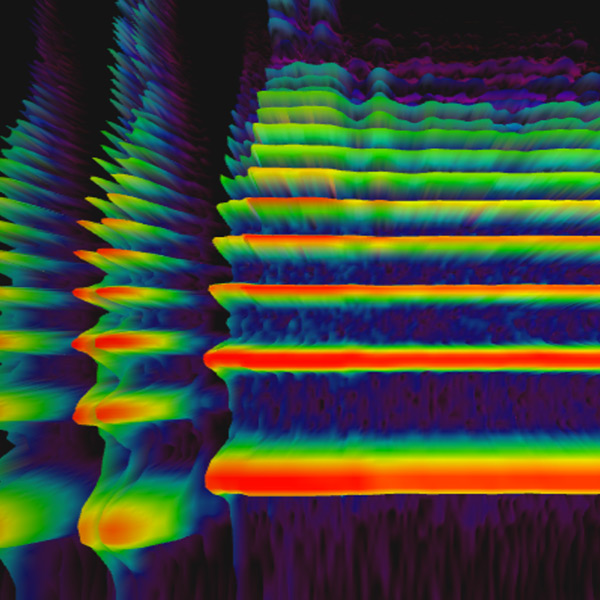
\includegraphics[height = 3cm]{spectrogram.jpeg}
%         \caption{ Time and Frequency Graph to see how the frequencies evolve over time}
%         \label{ fig:my_label}
%     \end{figure}
%     The above plot depicts a spectrogram which is obtained from passing a sound signal through a Gabor Transform, where it shows how the frequencies at any given point in time changes for the sound signal.
% \end{frame}

% \section[Frames and the Duality Principle]{Frames and the Duality Principle}

% \begin{frame}[fragile]{Frames}
%     In the previous cases, the operators could also be viewed as an inner product, of the input function with an orthonormal basis of $e^{-i\omega x}$ and $g(x)e^{-i \omega x}$ respectively as denoted below.

%     $$\mathscr{F}f (\omega) = \langle f, e^{-i \omega \cdot} \rangle$$
%     $$\mathscr{G}f (t, \omega) = \langle f(\cdot - t), e^{-i \omega \cdot} \rangle$$

%     However, we may not always want such a basis, since that is a strong condition, and we would like to reduce the condition of linear independence and orthonormality and thus introduce the concept of a frame!
% \end{frame}

% \begin{frame}[fragile]{More on Frames}
%     Orthonormal Bases have the desirable trait of 
% perfect reconstruction, that given an orthonormal basis $(x_n)_{n \in \mathbb{N}}$ we can reconstruct any arbitrary vector $x$, and the norm squared is the sum of coefficients:
%     $$x = \sum_{i = 1}^{n}{\langle x, x_i \rangle x_i}$$
%     $$\|x\|^2 = \sum_{i = 1}^{n}{\langle x, x_i \rangle}$$

%     Similarly \textbf{tight} frames keep both these properties with no requirements of orthonormality or linear independence. General frames are not as powerful but are useful nonetheless as they give you the norm within upper and lower bounds $A,B$ known as the frame bounds for a particular frame.
% \end{frame}

% \begin{frame}[fragile]{Duality Principle}
%     We can create an (underdetermined) matrix using the vectors of the frame as column vectors and take the adjoint (conjugate transpose) of that matrix. The columns of these vectors are (upto complex conjugation) the rows of our original matrix and the span of these vectors is known as the adjoint (or dual) space. 

%     This creates an idea for a duality principle where something in the original vector space has another representation in the dual space, and can be seen by looking at the rows of the original matrix.
% \end{frame}
% \section[Aim of the Capstone]{The Result}
% \begin{frame}[fragile]{The Result}
%     We aim to show the following result in the very specific case of a wandering vector:

%     \textbf{Let $\pi$ be a projective unitary representation of $G$ on $H$, with wandering vector $\psi$. Then $\eta\in H$ generates a (tight) frame if and only if it generates a(n orthonormal) Riesz basis.}
% \newline
% \newline
%     Note that this is related to the motivating example as the projective unitary representation mentioned here is closely related to systems of operators, (such as modulation and translation) as seen in the Gabor Transform which is a composition of a modulation and translation operator.
% \end{frame}


